The next result concerns connected graphs that can be decomposed into two
connected induced subgraphs with a path connecting them. With this in mind, we
introduce a construction based on paths. Let $L$ and $R$ be two connected
graphs on $m$ and $s$ vertices, respectively, where $m \le s$, and let~$P$ be a
path with $q$ vertices. Let $L \oplus_q R$ denote the graph obtained by adding
an edge between an endpoint of $P$ and a vertex of $L$ of degree not equal to
1, and an edge between the other endpoint of $P$ to a vertex of $R$ of degree
not equal to 1. Even though this definition depends on the choice of
attachment vertices, we will omit them in the notation, for our purpose is to
derive results that do not depend on them, apart from the fact that they do not
have degree 1 in $L$ and $R$. We remark that $m, s \ne 2$, since the only
connected graph on two vertices is $K_2$, whose vertices both have degree 1.
However, it is possible to have $m=1$ or $s=1$.

The vertices of $R$ are denoted as $r_1, \dots, r_s$, where they are sorted in
weakly increasing order of distance to the path $P$. In particular, $r_1$ is
attached to $P$, and $r_2$ and $r_3$ are neighbours of $r_1$ if $s\not=1$. A
similar notation is used for $L$; in particular $l_1$ is attached to $P$. Write
$L^* = L \setminus \{ l_1 \}$, $R^* = R \setminus \{ r_1 \}$, $P^* = P \cup
\{l_1, r_1\}$, and order the elements of the path as $p_1, \dots, p_q$ so that
$p_1$ is adjacent to $l_1$, and $p_q$ is adjacent to $r_1$; finally, we also
write $l_1 = p_0$ and $r_1 = p_{q+1}$. For instance, the graph $K_{3,1}
\oplus_4 C_4$ is illustrated in Figure~\ref{fig:oplus}.

\begin{figure}[ht]
\centering
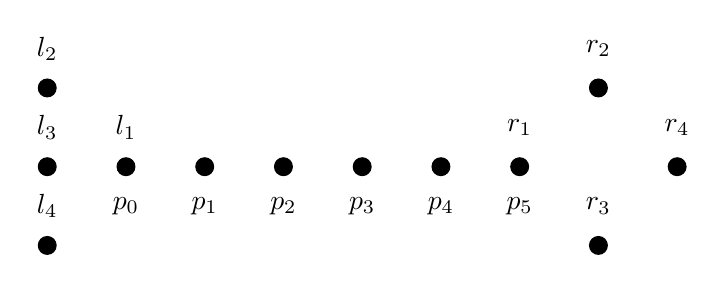
\begin{tikzpicture}[vertex/.style={circle, 
 draw, 
 fill=black,
 inner sep=0.08cm}]
	\node [vertex] (l1) at (1,1) {};
	\node [vertex] (l2) at (0,2) {};
	\node [vertex] (l3) at (0,1) {};
	\node [vertex] (l4) at (0,0) {};

	\node (ll1) at (1,1.5) {$l_1$};
	\node (ll2) at (0,2.5) {$l_2$};
	\node (ll3) at (0,1.5) {$l_3$};
	\node (ll4) at (0,0.5) {$l_4$};
	\node (pp0) at (1,0.5) {$p_0$};

	\node [vertex] (p1) at (2,1) {};
	\node [vertex] (p2) at (3,1) {};
	\node [vertex] (p3) at (4,1) {};
	\node [vertex] (p4) at (5,1) {};

	\node (pp1) at (2,0.5) {$p_1$};
	\node (pp2) at (3,0.5) {$p_2$};
	\node (pp3) at (4,0.5) {$p_3$};
	\node (pp4) at (5,0.5) {$p_4$};

	\node [vertex] (r1) at (6,1) {};
	\node [vertex] (r2) at (7,2) {};
	\node [vertex] (r3) at (8,1) {};
	\node [vertex] (r4) at (7,0) {};

	\node (rr1) at (6,1.5) {$r_1$};
	\node (rr2) at (7,2.5) {$r_2$};
	\node (rr3) at (8,1.5) {$r_4$};
	\node (rr4) at (7,0.5) {$r_3$};
	\node (pp5) at (6,0.5) {$p_5$};
	
 \edge{l1}{l2}
 \edge{l1}{l3}

 \edge{l1}{l4}

 \edge{l1}{p1}
 \edge{p1}{p2}
 \edge{p2}{p3}
 \edge{p3}{p4}
 \edge{p4}{r1}

 \edge{r1}{r2}
 \edge{r2}{r3}
 \edge{r3}{r4}
 \edge{r4}{r1}
\end{tikzpicture}
\caption{The graph $K_{3,1} \oplus_4 C_4$.} \label{fig:oplus}
\end{figure}
